\documentclass{standalone}

\usepackage{tikz}
\usetikzlibrary{positioning,arrows}
\usepackage{fontspec}
\setmainfont[Ligatures=TeX]{DM Mono}
\usepackage{calc}
\usepackage{xfp}
\usepackage{pgfmath,pgffor}

\def\letters{{"D","Y","K","T","M","M","T","M","M","T","M","M","D","Y","K","T","M","M","W","L","I","D","L","Y","I","K","T","M","M","T","M","M","T","M","M","Y"}}


\begin{document}
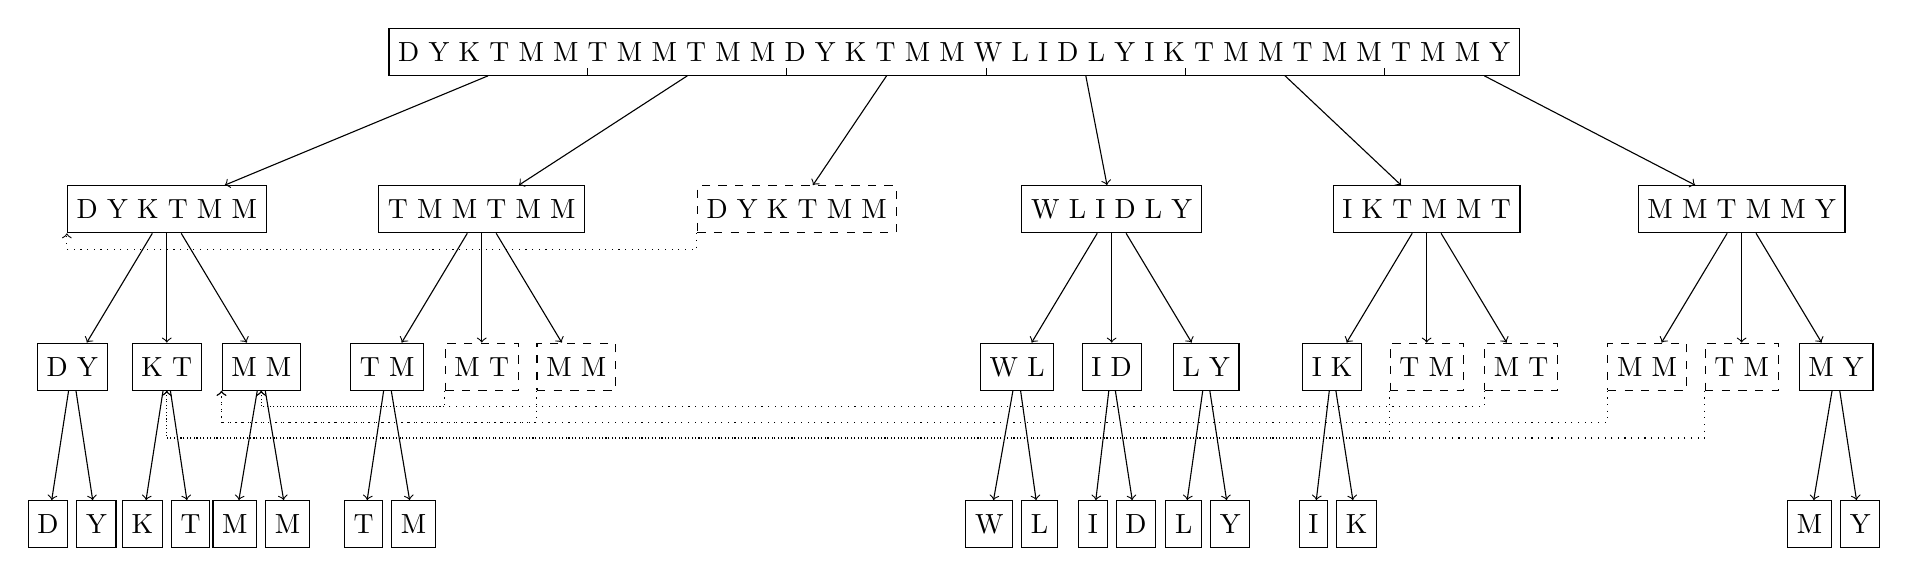
\begin{tikzpicture}[block/.style={draw,rectangle,minimum width=10pt,minimum height=1.7em},level/.style={sibling distance=40mm/#1},arrow/.style={draw=black, <-, shorten >=1pt}, edge from parent/.style={arrow}]
  \node[block] (root) at (0,0) {D Y K T M M T M M T M M D Y K T M M W L I D L Y I K T M M T M M T M M Y};

  \node[block] (l10) at (-10,-2) {D Y K T M M};
  \node[block] (l11) at (- 6,-2) {T M M T M M};
  \node[block,dashed] (l12) at (- 2,-2) {D Y K T M M};
  \node[block] (l13) at (  2,-2) {W L I D L Y};
  \node[block] (l14) at (  6,-2) {I K T M M T};
  \node[block] (l15) at ( 10,-2) {M M T M M Y};

  \foreach \n in {0,...,5}{
    \draw ([xshift=72pt * \n]root.south west) -- ++(0,3pt);  
    \draw[->] ([xshift=36pt + 72pt * \n]root.south west) -- (l1\n);  
  }

  \node[block] (l20) at (-11.2,-4) {D Y};
  \node[block] (l21) at (-10,-4) {K T};
  \node[block] (l22) at (-8.8,-4) {M M};
  \node[block] (l23) at (- 7.2,-4) {T M};
  \node[block, dashed] (l24) at (- 6,-4) {M T};
  \node[block,dashed] (l25) at (- 4.8,-4) {M M};
  %\node[block] (l26) at (- 3.2,-4) {D Y};
  %\node[block, dashed] (l27) at (- 2,-4) {K T};
  %\node[block] (l28) at (- 0.8,-4) {M M};
  \node[block] (l29) at (  0.8,-4) {W L};
  \node[block] (l210) at (  2,-4) {I D};
  \node[block] (l211) at (  3.2,-4) {L Y};
  \node[block] (l212) at (  4.8,-4) {I K};
  \node[block,dashed] (l213) at (  6,-4) {T M};
  \node[block,dashed] (l214) at (  7.2,-4) {M T};
  \node[block,dashed] (l215) at (  8.8,-4) {M M};
  \node[block,dashed] (l216) at ( 10,-4) {T M};
  \node[block] (l217) at ( 11.2,-4) {M Y};

  \foreach \i in {0,1,3,4,5} {
    \draw[->] (l1\i) -- (l2\inteval{3*\i});
    \draw[->] (l1\i) -- (l2\inteval{3*\i+1});
    \draw[->] (l1\i) -- (l2\inteval{3*\i+2});
  }

  \draw[->,dotted] (l12.south west) |- ++(0,-0.2cm) -| (l10.south west);
  \draw[->,dotted] (l24.south west) |- ++(0,-0.2cm) -| (l22);
  \draw[->,dotted] (l25.south west) |- ++(0,-0.4cm) -| (l22.south west);
  \draw[->,dotted] (l213.south west) |- ++(0,-0.6cm) -| (l21);
  \draw[->,dotted] (l214.south west) |- ++(0,-0.2cm) -| (l22);
  \draw[->,dotted] (l215.south west) |- ++(0,-0.4cm) -| (l22.south west);
  \draw[->,dotted] (l216.south west) |- ++(0,-0.6cm) -| (l21);

  \foreach \i in {0,1,2,3,9,10,11,12,17} {
    \node[block,below left=2 and 0.05 of l2\i.north] (l3\inteval{2*\i}) {
      \pgfmathparse{\letters[\inteval{2*\i}]}\pgfmathresult
    }; 
    \node[block,below right=2 and 0.05 of l2\i.north] (l3\inteval{2*\i+1}) {
      \pgfmathparse{\letters[\inteval{2*\i+1}]}\pgfmathresult
    }; 
    \draw[->] (l2\i) -- (l3\inteval{2*\i});
    \draw[->] (l2\i) -- (l3\inteval{2*\i+1});
  }


\end{tikzpicture}
\end{document}


